\documentclass[t, 10pt, handout, aspectratio=169]{beamer}
\usepackage{lipsum}
\usepackage{tikz}
\usepackage{pgfplots, pgfplotstable}
\usepackage{booktabs}
\usepackage{amsmath,bm,amstext}
\usepackage{mdframed}


\pgfplotsset{compat=1.14}

%\usetheme[framenumber,totalframenumber]{QU}
\usetheme[color=blue,framenumber,totalframenumber, footline, footertext]{KU}


\title[Introduction to Tensor]{Introduction to \texttt{Tensor}}
\subtitle{Intelligent Computing for Computational Intelligence \\
in post Moore’s Law era!}

\author[yanglet]{Xiao-Yang Liu\\
\url{www.tensorlet.com}}
\institute[CU]{Columbia University}

\footertext{\textcolor{red}{\url{www.tensorlet.com}}}


\date[\number\month/\number\day/\number\year]{\today}


\begin{document}

\begin{frame}
  \titlepage
\end{frame}

\begin{frame}{Agenda}
\begin{itemize}
    \large \item \textcolor{red}{Background}
    \large \item {Tensor Decompositions (CP, Tucker, and Tensor-Train/Tensor-Ring)}
    \large \item{Transform-based Tensor Model and Applications}
    \large \item{Tensor Computations (cuTensor, TensorDeC$++$)}
\end{itemize}
\end{frame}

\begin{frame}{Background}
\large Multidimensional data of exceedingly huge volume, variety and structural richness become ubiquitous across disciplines in engineering and data science:
\begin{itemize}
    \item multimedia data like speech and video
    \item remote sensing data
    \item medical and biological data
    \item seismic data
\end{itemize}
\vskip 0.2\margin
\large Some data can have more meaningful representation using multi-way arrays -- \textbf{tensor}, rather than matrices (two-way arrays).
\end{frame}

\begin{frame}{What is tensor?}
\vskip -1ex
\begin{figure}
	\centering  
	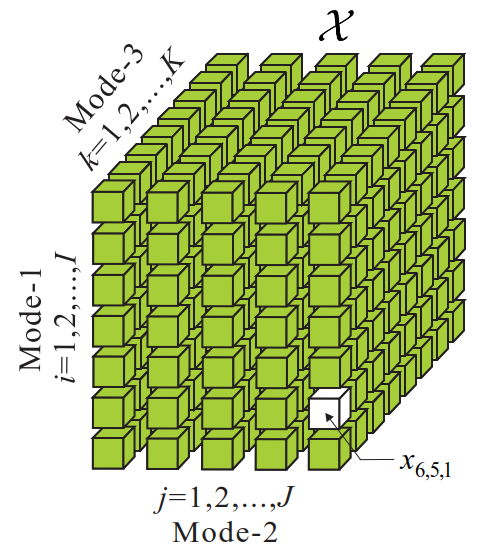
\includegraphics[height=0.7\paperheight]{figs/tensor_shape}
	\label{fig:tensor_shape}
\end{figure}
\end{frame}

\begin{frame}{What is tensor?}
\vskip -1ex
\begin{figure}
	\centering  
	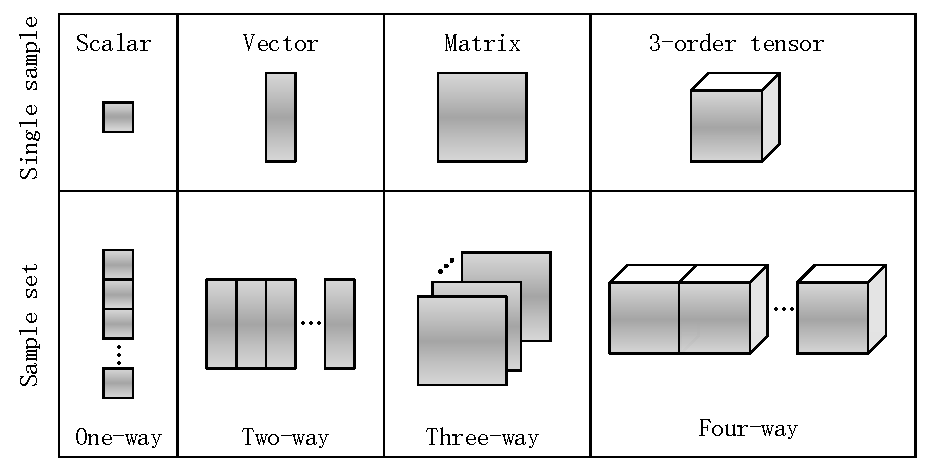
\includegraphics[height=0.8\paperheight]{figs/tensor_sample}
	\label{fig:tensor_sample}
\end{figure}
\end{frame}

\begin{frame}{Tensor fibers}
\vskip -3ex
\begin{figure}
	\centering  
	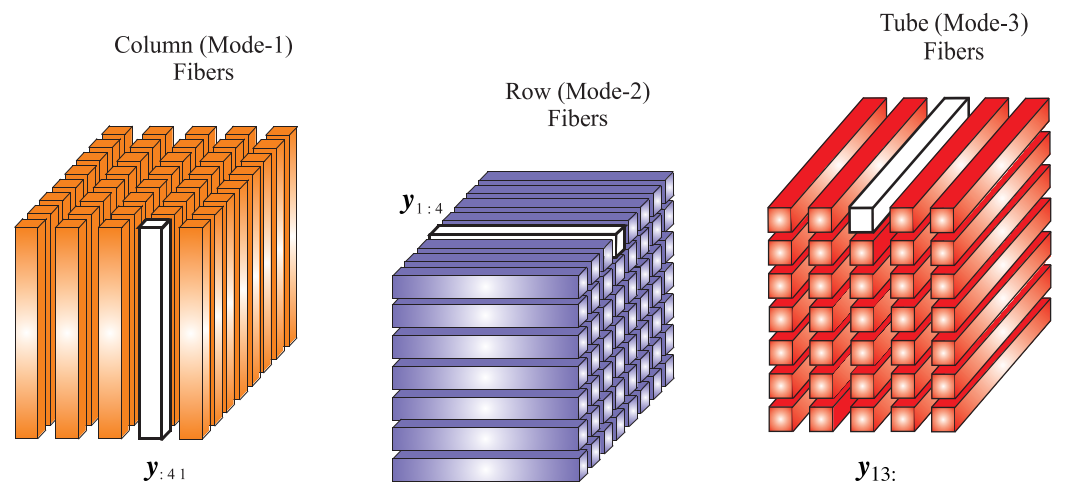
\includegraphics[width=\linewidth]{figs/tensor_fibers}
	\label{fig:tensor_fibers}
\end{figure}
\end{frame}

\begin{frame}{Tensor slices}
\begin{figure}
	\centering  
	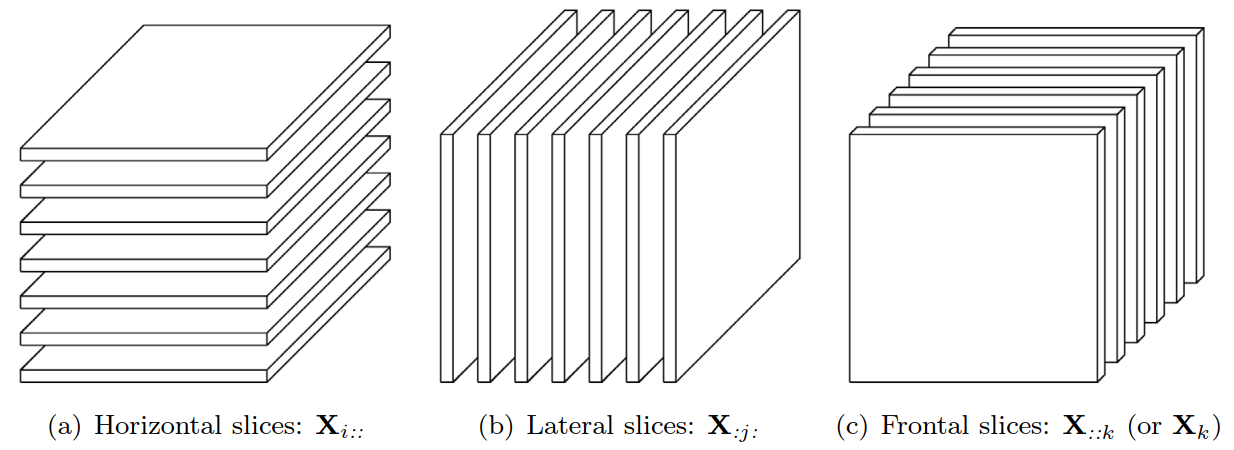
\includegraphics[width=\linewidth]{figs/tensor_slices}
	\label{fig:tensor_slices}
\end{figure}
\end{frame}

\begin{frame}{Tensor unfolding}
\vskip -3ex
\begin{columns}[c]  %开始进入分栏环境,居中设置
\column{0.4\linewidth}  
\begin{figure}
	\centering  
	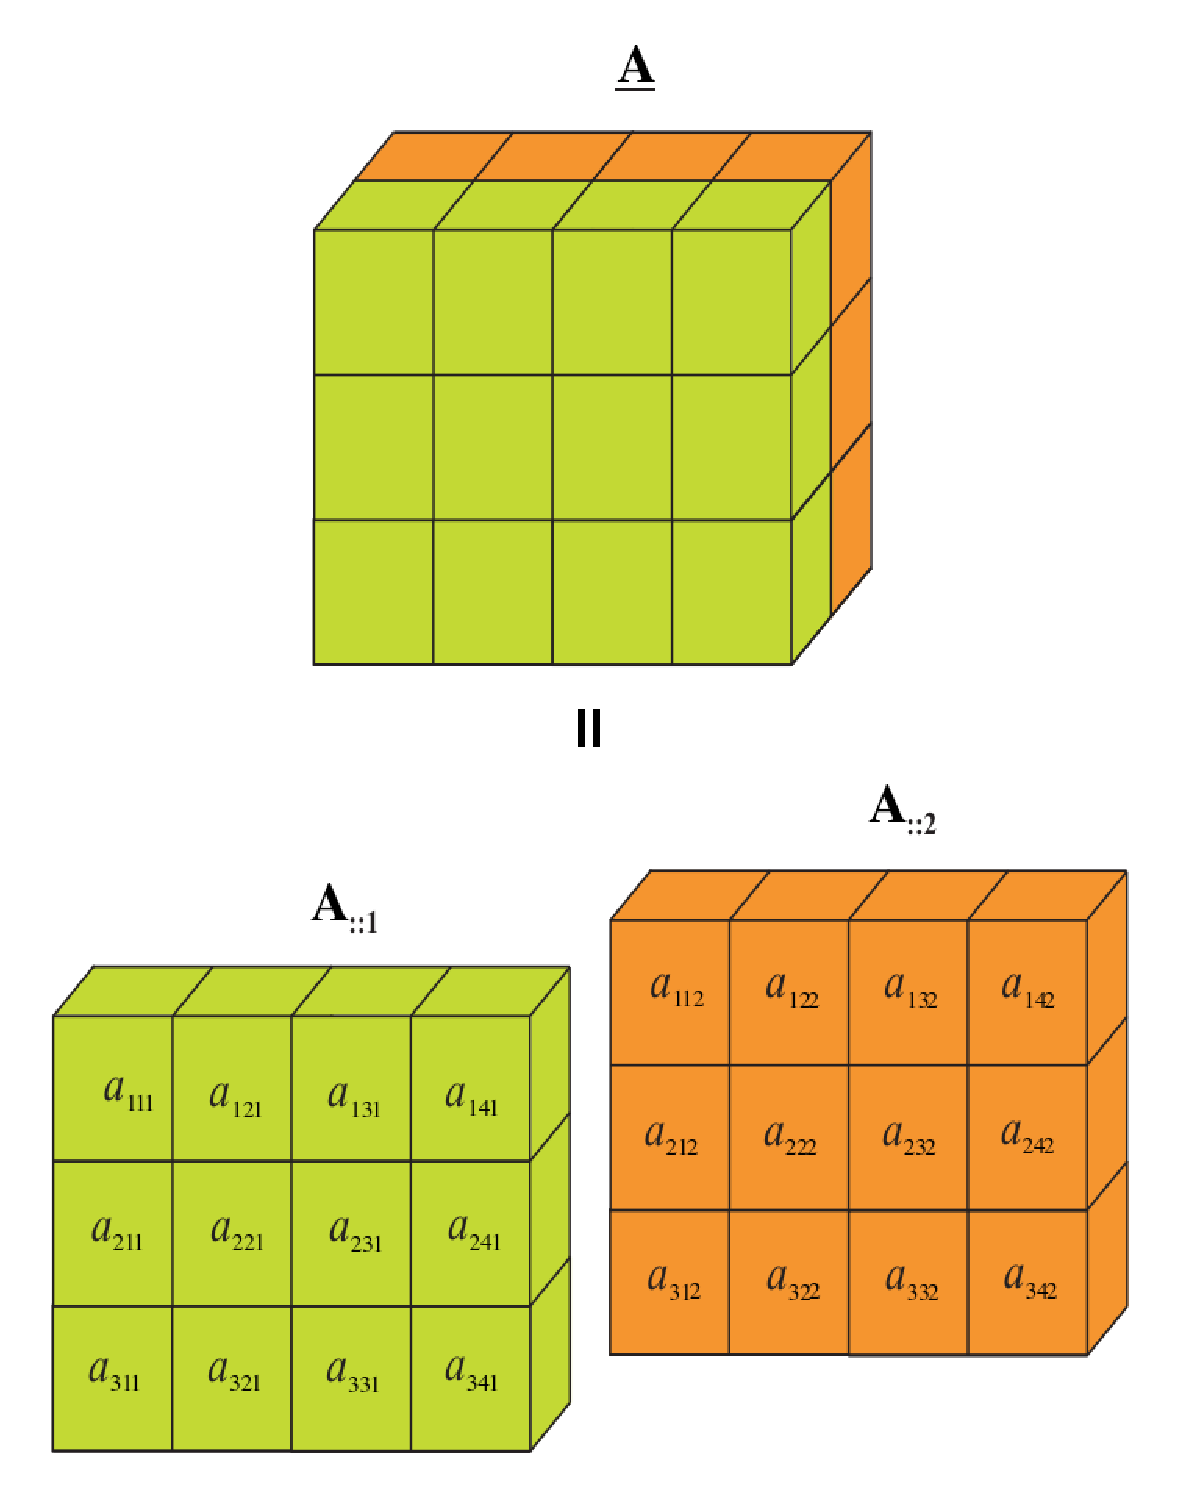
\includegraphics[height=0.75\paperheight]{figs/tensor_unfolding}
	\label{fig:tensor_unfolding}
\end{figure}

\column{0.6\linewidth}  
\begin{figure}
	\centering  
	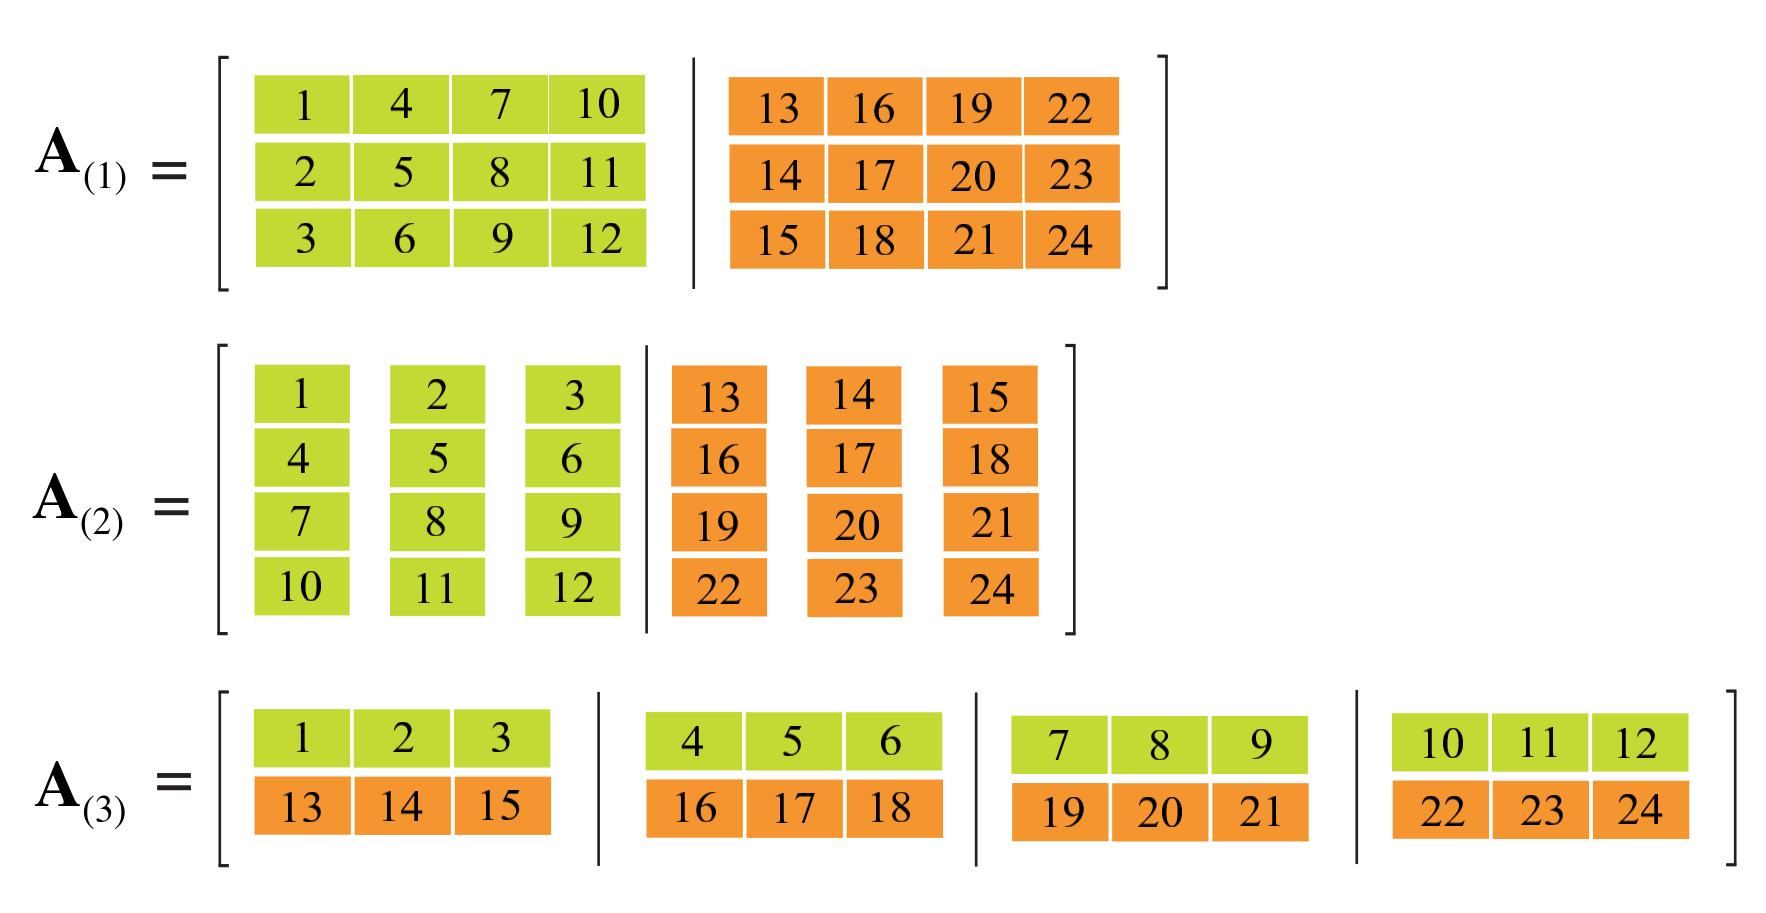
\includegraphics[width=\linewidth]{figs/tensor_unfolding2}
	\label{fig:tensor_unfolding2}
\end{figure}
\centering
$\mathbf{A}_{(i)}$ means mode-$i$ unfolding.
\end{columns}  %分栏环境结束

\end{frame}



\begin{frame}{Agenda}
\begin{itemize}
    \large \item {Background}
    \large \item \textcolor{red}{Tensor Decompositions (CP, Tucker, and Tensor-Train/Tensor-Ring)}
    \large \item{Transform-based Tensor Model and Applications}
    \large \item{Tensor Computations (cuTensor, TensorDeC$++$)}
\end{itemize}
\end{frame}

\begin{frame}{CP Decomposition}
\vskip -1ex
\begin{figure}[t]
	\centering  
	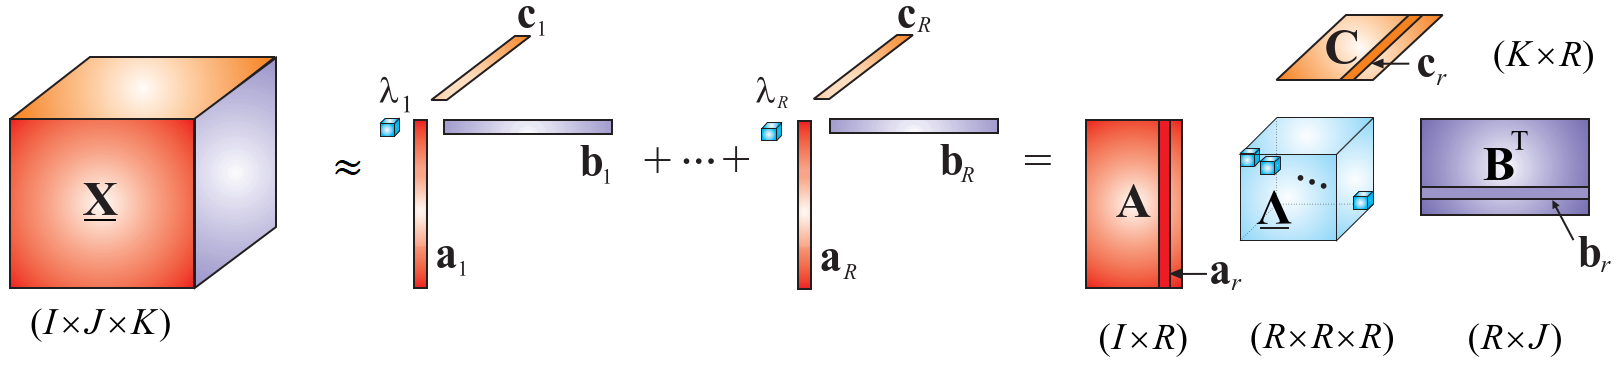
\includegraphics[width=\linewidth]{figs/cp_arch}
	\label{fig:cp_arch}
\end{figure}
\begin{columns}
\column{0.5\linewidth}
\vskip -10ex
\begin{align*}
\underline{\mathbf{X}}&\approx\sum_{r=1}^{R}\lambda_{r}\mathbf{b}_{r}^{(1)}\circ\mathbf{b}_{r}^{(2)}\circ\cdots\circ\mathbf{b}_{r}^{(N)} \\
&=\underline{\mathbf{\Lambda}}\times_{1}\mathbf{B}^{(1)}\times_{2}\mathbf{B}^{(2)}\cdots\times_{N}\mathbf{B}^{(N)} \\
&=[\![\mathbf{\Lambda};\mathbf{B}^{(1)},\mathbf{B}^{(1)},\cdots,\mathbf{B}^{(N)}]\!]
\end{align*}

\column{0.5\linewidth}
\vskip -8ex
\begin{align*}
\mathbf{X}_{(1)}&=\mathbf{A}\mathbf{\Lambda}(\mathbf{C}\odot\mathbf{B})^{T}+\mathbf{E}_{(1)} \\
\mathbf{X}_{(2)}&=\mathbf{B}\mathbf{\Lambda}(\mathbf{C}\odot\mathbf{A})^{T}+\mathbf{E}_{(2)} \\
\mathbf{X}_{(3)}&=\mathbf{C}\mathbf{\Lambda}(\mathbf{B}\odot\mathbf{A})^{T}+\mathbf{E}_{(3)}
\end{align*}

\end{columns}
\end{frame}

\begin{frame}{CP Decomposition}
\large
\begin{table}
\begin{tabular}{l | l}
Name & Proposed by \\
\hline \hline
Polyadic form of a tensor & Hitchcock, 1927 \\ 
PARAFAC (parallel factors) & Harshman, 1970\\
CANDECOMP or CAND (canonical decomposition) & Carroll and Chang, 1970\\
Topographic components model & Mocks, 1988 \\
CP (CANDECOMP/PARAFAC) & Kiers, 2000
\end{tabular}
\caption{Some of the many names for the CP decomposition.}
\end{table}
\end{frame}

\begin{frame}{Tucker Decomposition}
\vskip -2ex
\begin{figure}[t]
	\centering  
	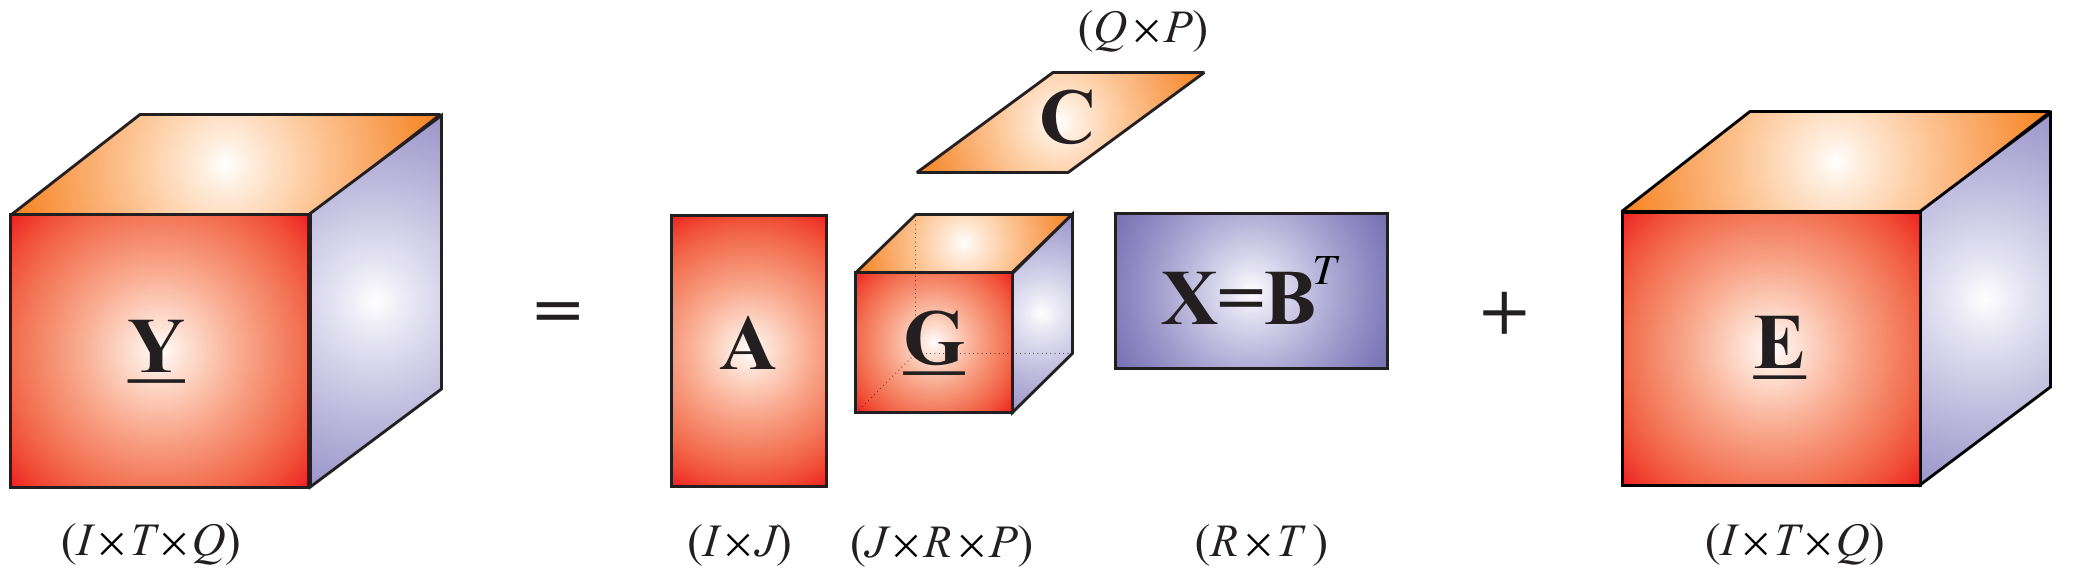
\includegraphics[width=0.95\linewidth]{figs/tucker_arch}
	\label{fig:tucker_arch}
\end{figure}
\vskip -2.5ex
\begin{mdframed}[backgroundcolor=brown!20,roundcorner=8pt,leftmargin=60pt,rightmargin=60pt]
\centering
$
\underline{\mathbf{Y}}=\underline{\mathbf{G}}\times_{1}\mathbf{A}\times_{2}\mathbf{B}\times_{3}\mathbf{C}+\mathbf{E}=[\![\mathbf{G};\mathbf{A},\mathbf{B},\mathbf{C}]\!]+\underline{\mathbf{E}}
$
\end{mdframed}
\vskip -0.5ex
\begin{align*}
\mathbf{X}_{(1)}&\approx\mathbf{A}\mathbf{G}_{(1)}(\mathbf{C}\otimes\mathbf{B})^{T}\\
\mathbf{X}_{(2)}&\approx\mathbf{B}\mathbf{G}_{(2)}(\mathbf{C}\otimes\mathbf{A})^{T}\\
\mathbf{X}_{(3)}&\approx\mathbf{C}\mathbf{G}_{(3)}(\mathbf{B}\otimes\mathbf{A})^{T}
\end{align*}
\end{frame}

\begin{frame}{Tucker Decomposition}
\large
\begin{table}
\begin{tabular}{l | l}
Name & Proposed by \\
\hline \hline
Three-mode factor analysis (3MFA/Tucker3) & Tucker, 1966 \\ 
Three-mode PCA (3MPCA) &  Kroonenberg and De Leeuw, 1980\\
N-mode PCA & Kapteyn et al., 1986 \\
Higher-order SVD (HOSVD)  & De Lathauwer et al., 2000 \\
N-mode SVD & Vasilescu and Terzopoulos, 2002
\end{tabular}
\caption{Names for the Tucker decomposition (some specific to three-way and some for N-way).}
\end{table}
\end{frame}

\begin{frame}{Tensor Train Decomposition}
\large
\begin{block}{Low-rank Decomposition}
$$
\begin{aligned}
&\mathbf{A}=\mathbf{G}_{1}\mathbf{G}_{2}  \\
&\mathbf{G}_{1}\text{: collection of rows, }\mathbf{G}_{2}\text{: collection of columbs}\\
&\mathbf{A}_{i_1i_2}=\underbrace{\mathbf{G}_1(i_1)}_{1\times R}\underbrace{\mathbf{G}_2(i_2)}_{R\times 1}
\end{aligned}
$$
\end{block}
\begin{figure}
	\centering  
	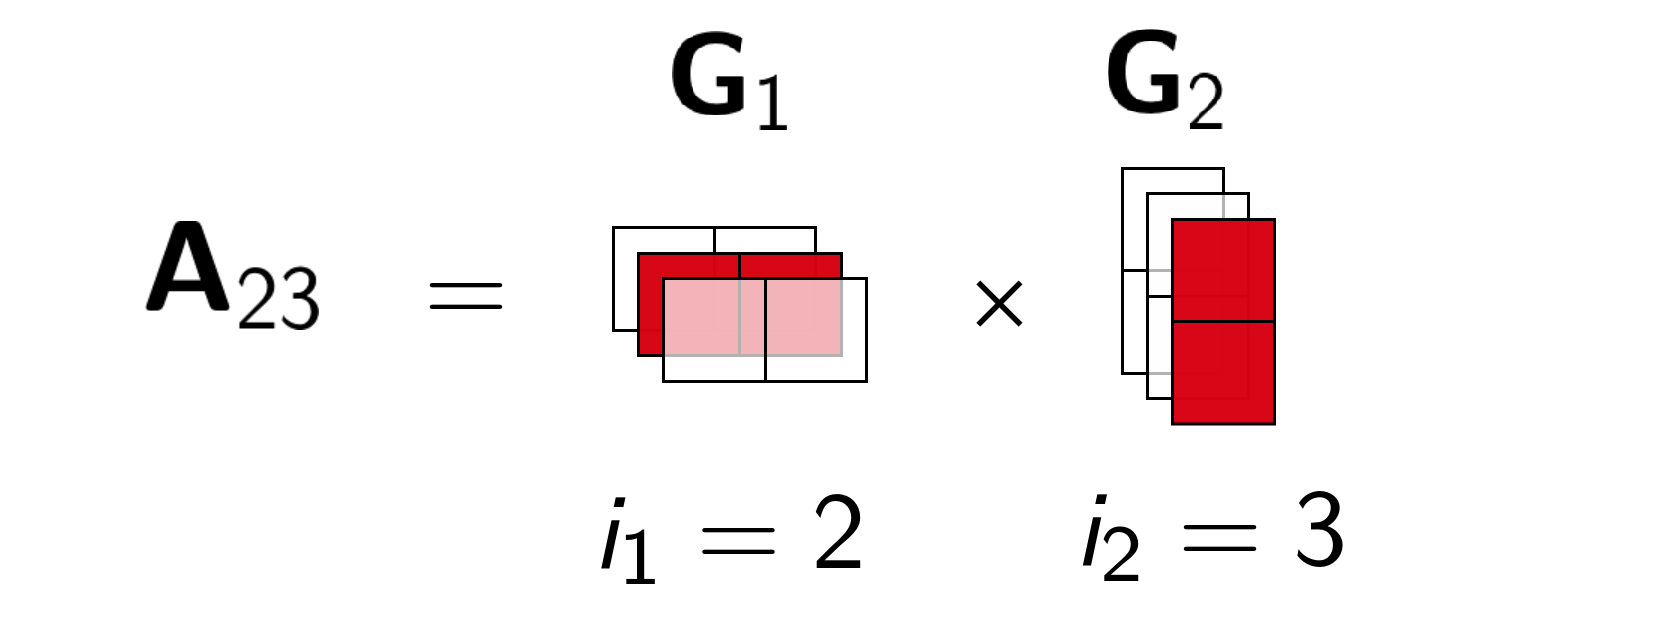
\includegraphics[width=0.45\linewidth]{figs/tt_lowrank.png}
	\label{fig:tt_lowrank}
\end{figure}
\end{frame}

\begin{frame}{Tensor Train Decomposition}
\large
\begin{block}{TT Form}
$$
\underline{\mathbf{A}}_{i_1i_2\cdots i_N}=\underbrace{\mathbf{G}_{1}(i_1)}_{1\times R}\underbrace{\mathbf{G}_{2}(i_2)}_{R\times R}\cdots\underbrace{\mathbf{G}_{N}(i_N)}_{R\times 1}
$$
\end{block}
\begin{figure}
	\centering  
	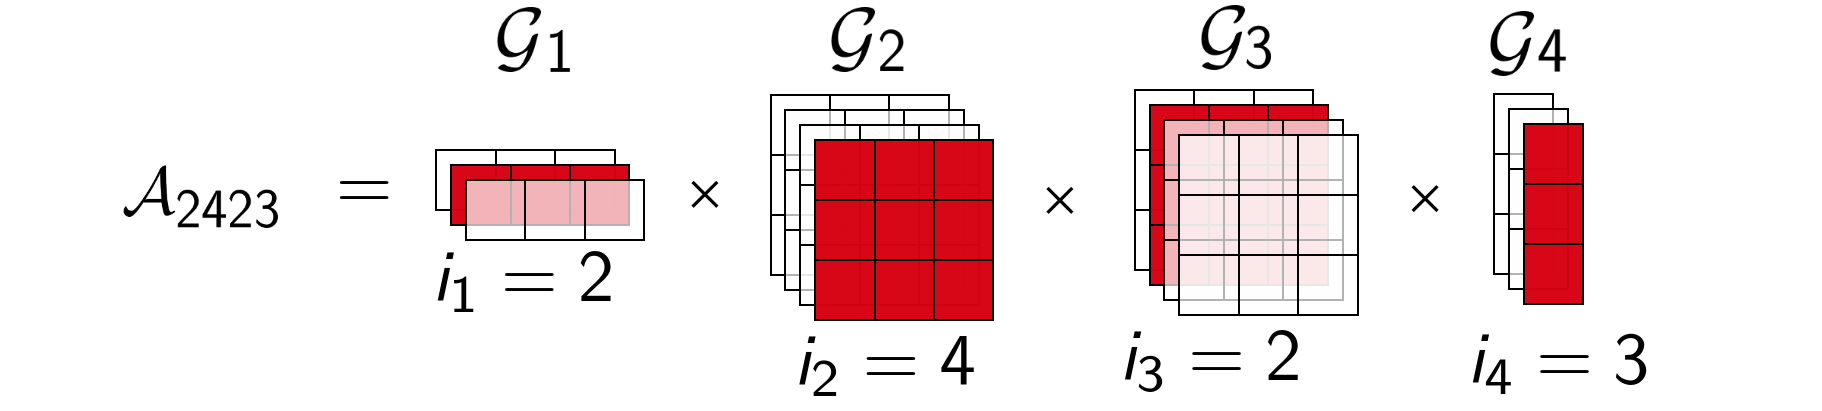
\includegraphics[width=0.9\linewidth]{figs/tt_form_example.png}
	\label{fig:tt_form_example}
\end{figure}
\end{frame}

\begin{frame}{Tensor Ring Decomposition}
\large

\begin{block}{TR Form}
$$
\begin{aligned}
\underline{\mathbf{A}}_{i_1i_2\cdots i_N}=\text{Tr}\{\mathbf{Z}_1(i_1)\mathbf{Z}_2(i_2)\cdots\mathbf{Z}_N(i_N)\}
=\text{Tr}\left\{\prod_{k=1}^{N}\mathbf{Z}_k(i_k)\right\}
\end{aligned}
$$
\end{block}
\begin{figure}
	\centering  
	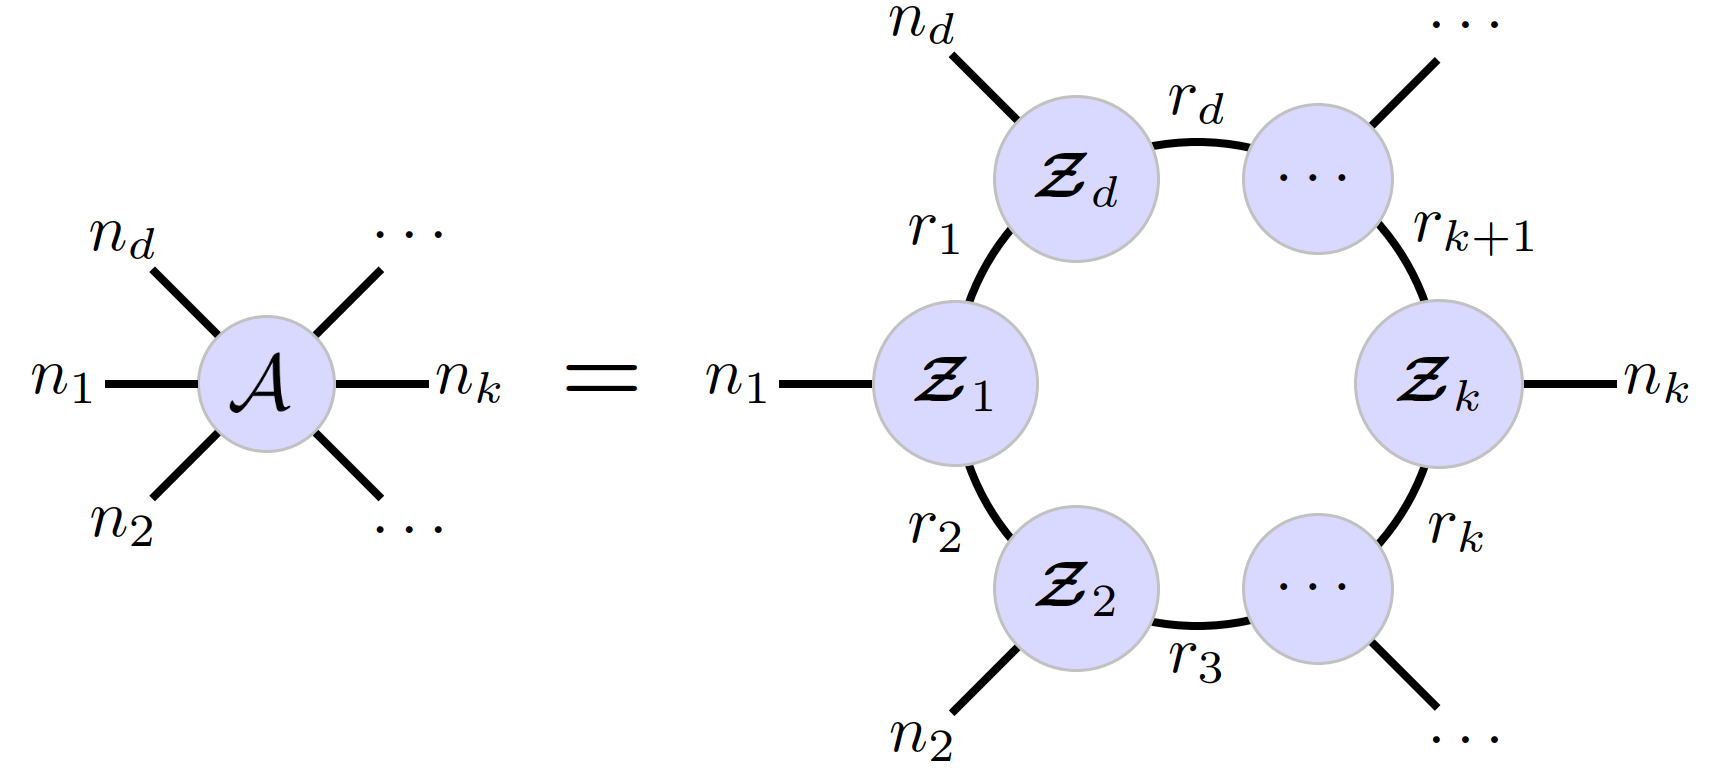
\includegraphics[width=0.55\linewidth]{figs/tensor_ring_arch.png}
	\label{fig:tensor_ring_arch}
\end{figure}
\end{frame}

\begin{frame}{Agenda}
\begin{itemize}
    \large \item {Background}
    \large \item {Tensor Decompositions (CP, Tucker, and Tensor-Train/Tensor-Ring)}
    \large \item \textcolor{red}{Transform-based Tensor Model and Applications}
    \large \item{Tensor Computations (cuTensor, TensorDeC$++$)}
\end{itemize}
\end{frame}

\begin{frame}{Low-tubal-rank Model}
\vskip -1ex
\begin{block}{Notation}
\vskip -1ex
$$
\texttt{bcirc}(\mathcal{A})=\left[
  \begin{matrix}
   A^{(1)} & A^{(n)} & A^{(n-1)} & \cdots &A^{(2)} \\
   A^{(2)} & A^{(1)} & A^{(n)} & \cdots &A^{(3)} \\
   \vdots & \vdots & \vdots & \ddots & \vdots \\
    A^{(n)} & A^{(n-1)} & \cdots &A^{(2)} & A^{(1)}
  \end{matrix}
  \right]
$$
$$
\texttt{unfold}(\mathcal{A})=\left[
  \begin{matrix}
    A^{(1)} \\
    A^{(2)} \\
    \vdots \\
    A^{(n)}
  \end{matrix}
\right], ~~~~~~~~\texttt{fold}(\texttt{unfold}(\mathcal{A}))=\mathcal{A}
$$
\end{block}
\end{frame}

\begin{frame}{Low-tubal-rank Model}
\begin{block}{Notation}
~~~~For $\mathcal{A}\in\mathbb{R}^{l\times m\times n}$ 
$$\mathcal{X}^{(l)}\equiv\mathcal{X}(:,:,l),~~~~\vec{\mathcal{A}}_i\equiv\mathcal{A}(:,i,:),~~~~\mathcal{A}^{(j)}\equiv\mathcal{A}(:,:,j)$$
$$\hat{\mathcal{A}} := \texttt{fft}(\mathcal{A}, [], 3)$$
\end{block}
\end{frame}

\begin{frame}{Low-tubal-rank Model}
\begin{block}{Definetion. t-Product}
$$\mathcal{A}*\mathcal{B}=\texttt{fold}(\texttt{bcirc}(\mathcal{A})\cdot\texttt{unfold}(\mathcal{B}))$$
\end{block}
\begin{block}{Observation}
~~~~Given $\mathbf{a}, \mathbf{b} \in \mathbb{K}_n$, $\mathbf{a} * \mathbf{b}$ can be computed as
$$
\mathbf{a} * \mathbf{b} := \texttt{ifft}(\hat{\mathbf{a}} \odot \hat{\mathbf{b}}, [], 3),
$$
where $\odot$ of two tubal scalars means pointwise multiplication.\\
~~~~Factorizations of $\mathcal{A}$ are created (implicitly) by applying the appropriate matrix factorization to each of the $\hat{\mathcal{A}}^{(i)}$
$$
\mathcal{A}=\mathcal{Q} * \mathcal{R} \Longleftrightarrow \hat{\mathcal{A}}^{(i)}=\hat{\mathcal{Q}}^{(i)}\hat{\mathcal{R}}^{(i)}.
$$
\end{block}
\end{frame}

\begin{frame}{Low-tubal-rank Model}
\begin{block}{t-SVD}
$$
\mathcal{A}=\mathcal{U}*\mathcal{S}*\mathcal{V}^{T}=\sum_{i=1}^{\text{min}(l,m)}\vec{\mathcal{U}}_i*\mathbf{s}_i*\vec{\mathcal{V}}_i^T, ~~~~\mathbf{s}_i :=\mathcal{S}(i,i,:)
$$
\end{block}
\vskip -1.5ex
\begin{figure}
	\centering  
	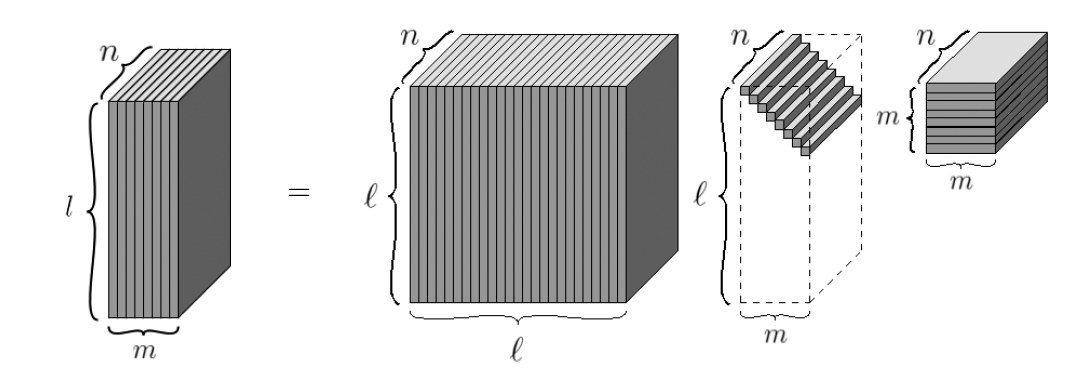
\includegraphics[width=0.7\linewidth]{figs/tsvd_arch.png}
	\label{fig:tsvd_arch}
\end{figure}
\end{frame}

\begin{frame}{Tubal-Tensor Sparse Coding}
\large
\begin{mdframed}[backgroundcolor=brown!20,roundcorner=8pt,leftmargin=60pt,rightmargin=60pt]
$$
\begin{aligned}
\min_{\mathcal{D},\mathcal{C}}&~~~\frac{1}{2}\|\mathcal{A}-\mathcal{D}*\mathcal{C}\|_{F}^{2}+\beta\|\mathcal{C}\|_1 \\
\text{s.t.} &~~~ \|\vec{\mathcal{D}}_j\|_F^2\le 1, j=1,2,\cdots,r
\end{aligned}
$$
$$\text{where}~\mathcal{D}\in\mathbb{R}^{l\times r\times n} ~\text{and} ~r > l$$
\end{mdframed}
\end{frame}

\begin{frame}{Tubal-Tensor Sparse Coding}
\begin{block}{Tensor Coefficients Learning}
$$
\min_{\mathcal{C}}:=f(\mathcal{C})+\beta g(\mathcal{C})
$$
$$
f(\mathcal{C}) = \frac{1}{2}\|\mathcal{A}-\mathcal{D}*\mathcal{C}\|_F^2, ~~g(\mathcal{C}) = \|\mathcal{C}\|_1
$$
\end{block}
\end{frame}

\begin{frame}{Tubal-Tensor Sparse Coding}
\begin{block}{Tensor Dictionary Learning}
\vskip -1ex
$$
\begin{aligned}
\min_{\mathcal{D}}&~~~\frac{1}{2}\|\mathcal{A}-\mathcal{D}*\mathcal{C}\|_{F}^{2}+\beta\|\mathcal{C}\|_1 \\
\text{s.t.} &~~~ \|\vec{\mathcal{D}}_j\|_F^2\le 1, j=1,2,\cdots,r.
\end{aligned}
$$
~~~~We transform this problem into the frequecy domain:
\vskip -1ex
$$
\begin{aligned}
\min_{\hat{\mathcal{D}}^{(l)}}&~~~\sum_{l=1}^{n}\|\hat{\mathcal{X}}^{(l)}-\hat{\mathcal{D}}^{(l)}\hat{\mathcal{C}}^{(l)}\|_F^2,l=1,2,\cdots,n \\
\text{s.t.}&~~~\sum_{l=1}^{n}\|\hat{\mathcal{D}}^{(l)}(:,j)\|_F^2\le n, j=1,2,\cdots,r.
\end{aligned}
$$
~~~~Then adopt the Lagrange dual (Lee et al. 2007) to solve the dual variables by Newton’s algorithm.
\end{block}
\end{frame}

\begin{frame}{Tubal-Tensor Sparse Coding}
\begin{figure}
	\centering  
	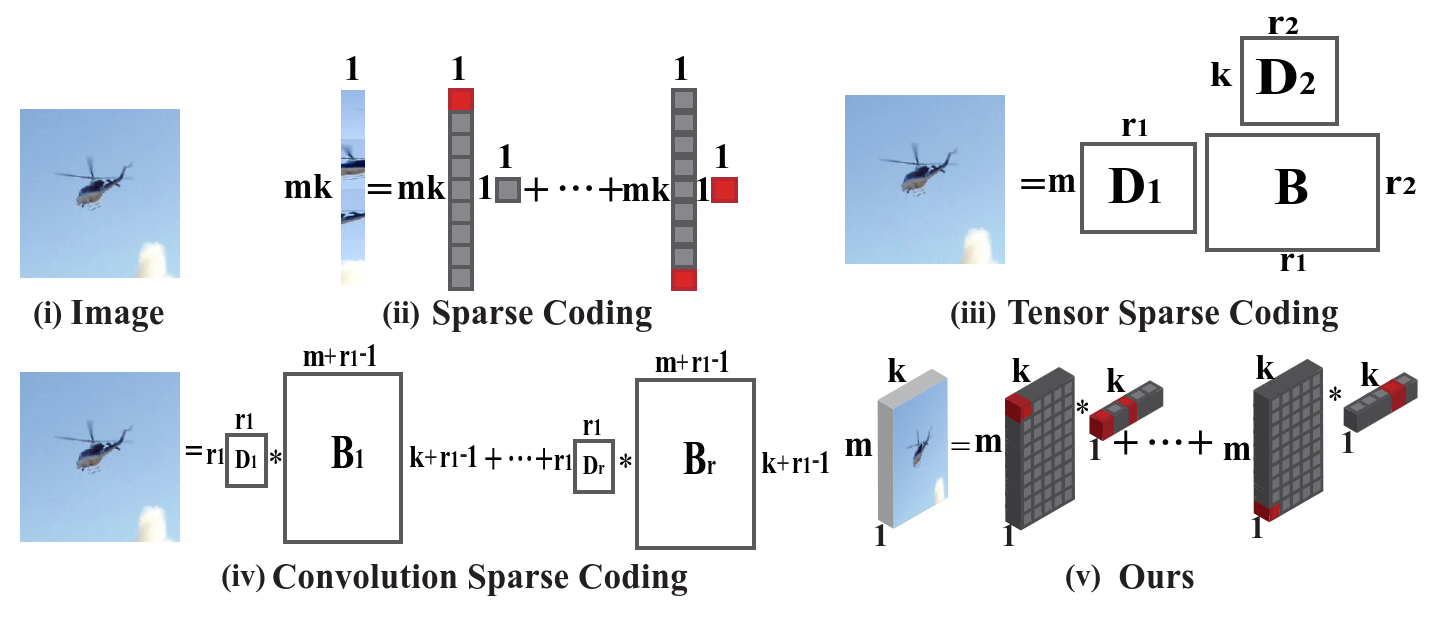
\includegraphics[width=0.9\linewidth]{figs/2dsc_arch.png}
	\label{fig:2dsc_arch}
\end{figure}
\end{frame}

\begin{frame}{Agenda}
\begin{itemize}
    \large \item {Background}
    \large \item {Tensor Decompositions (CP, Tucker, and Tensor-Train/Tensor-Ring)}
    \large \item {Transform-based Tensor Model and Applications}
    \large \item \textcolor{red}{Tensor Computations (cuTensor, TensorDeC$++$)}
\end{itemize}
\end{frame}

\begin{frame}{cuTensor-tubal (GPU)}
\large
This library is a general approach to compute low-tubal-rank tensor operations in the frequency domain on GPUs.
\begin{enumerate}
  \item Obtain the frequency domain representation of the input tensor by performing Fourier transform along the third dimension (called tube-wise DFT) on the GPU;
  \item In the frequency domain, the tensor operations are separated into multiple independent complex matrix computations that possess strong parallelism;
  \item Converting the frequency domain results back to the time domain through inverse Fourier transform along the third dimension on the GPU (called tube-wise inverse DFT).
\end{enumerate}
\end{frame}

\begin{frame}{cuTensor-tubal (GPU)}

\begin{table}
$\begin{array}{l | l | l}
\text{Operation} & \text{Input} & \text{Output} \\
\hline \hline
\text{t-FFT} & \mathcal{A}\in\mathbb{R}^{m\times n\times k} & \tilde{\mathcal{A}}\in\mathbb{C}^{m\times n\times k} \\
\text{inverse t-FFT} & \tilde{\mathcal{A}}\in\mathbb{C}^{m\times n\times k} & \mathcal{A}\in\mathbb{R}^{m\times n\times k} \\
\text{t-product} & \mathcal{A}\in\mathbb{R}^{m\times l\times k},\mathcal{B}\in\mathbb{R}^{l\times n\times k} & \mathcal{C}\in\mathbb{R}^{m\times n\times k} \\
\text{t-SVD} & \mathcal{T}\in\mathbb{R}^{m\times n\times k} & \mathcal{U}\in\mathbb{R}^{m\times m\times k},\mathcal{V}\in\mathbb{R}^{n\times n\times k}, \mathcal{\Theta}\in\mathbb{R}^{m\times n\times k} \\
\text{t-QR} & \mathcal{T}\in\mathbb{R}^{m\times n\times k} & \mathcal{Q}\in\mathbb{R}^{m\times m\times k}, \mathcal{R}\in\mathbb{R}^{m\times n\times k} \\
\text{t-inverse} &\mathcal{T}\in\mathbb{R}^{n\times n\times k} &\mathcal{T}^{-1}\in\mathbb{R}^{n\times n\times k} \\
\text{t-normalization} & \mathcal{T}\in\mathbb{R}^{m\times 1\times k} & \mathcal{T}\in\mathbb{R}^{m\times 1\times k}
\end{array}$
\caption{Seven tensor operations in the cuTensor-tubal library}
\end{table}


\end{frame}

\begin{frame}{cuTensor-tubal (GPU)}
\begin{figure}
	\centering  
	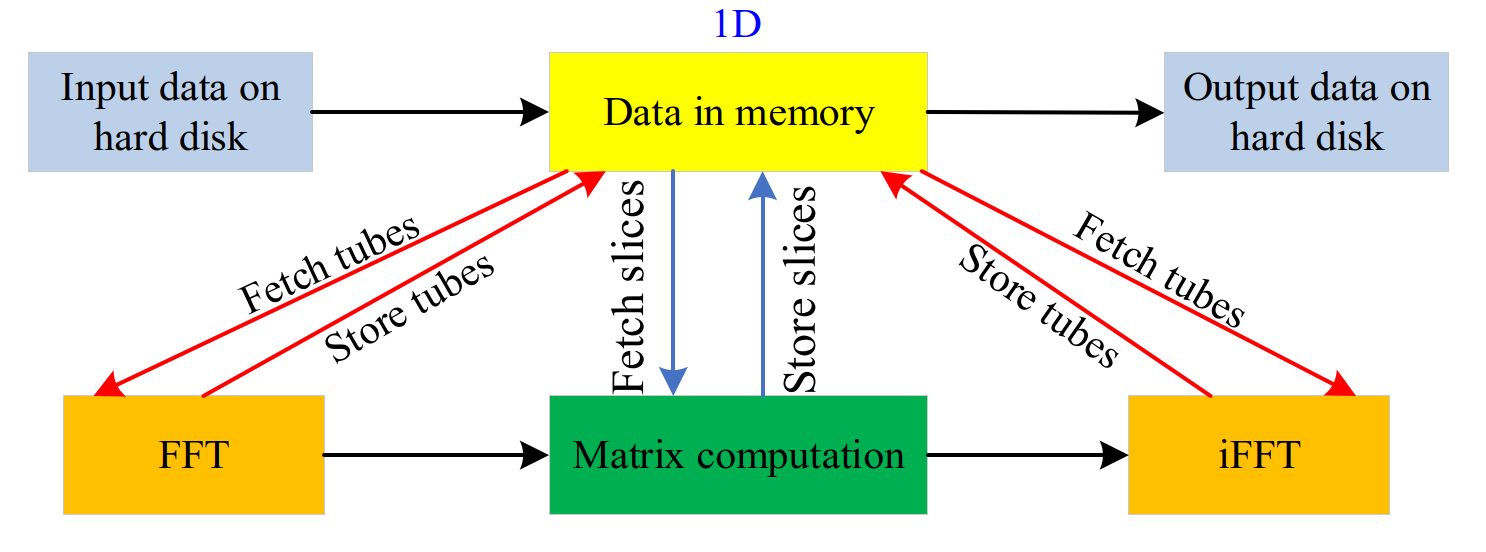
\includegraphics[width=0.55\linewidth]{figs/cutensor_datastructure.png}\\
	Data structures in tensor computations
	\label{fig:cutensor_datastructure}
\end{figure}
\begin{figure}
	\centering  
	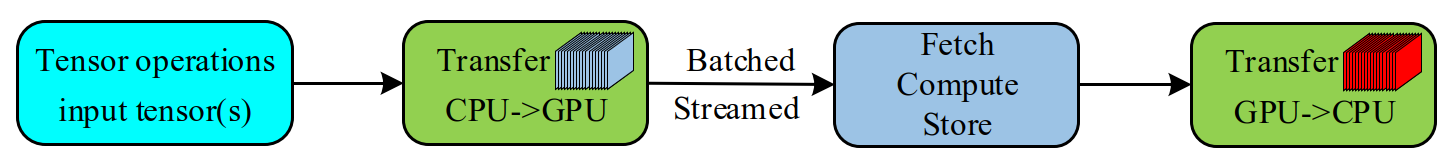
\includegraphics[width=0.9\linewidth]{figs/cutensor_workflow.png}\\
	System workflow of the cuTensor-tubal library
	\label{fig:cutensor_workflow}
\end{figure}
\end{frame}

\end{document}
